\begin{figure}[h]
	\centering
	\label{fig:bit_patterns}
	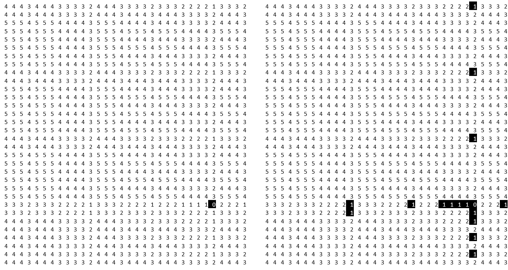
\includegraphics[width=3.5in]{contents/img/0-1}\vspace*{5pt}
	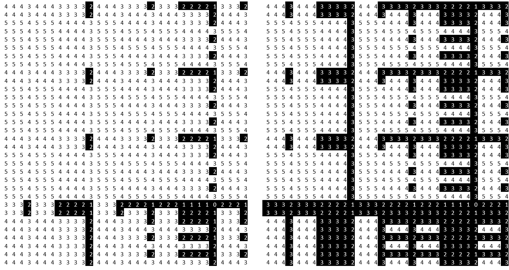
\includegraphics[width=3.5in]{contents/img/2-3}\vspace*{5pt}
	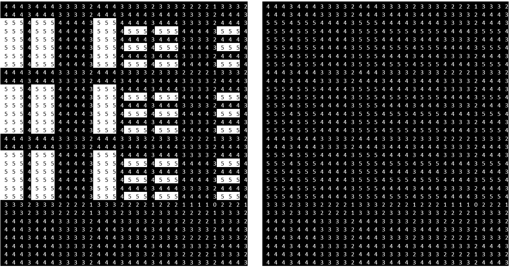
\includegraphics[width=3.5in]{contents/img/4-5}
	\caption{Bit patterns followed by blocks of size $4^{5}=32\times32$ in the bit-based representation of $\mathcal{N}(\texttt{acgtacgtacgt},5)$. Black signifies a 1. There are $(5+2)=7$ possible patterns---the empty pattern (all 0s) is not shown.}
\end{figure}